\documentclass[notes,11pt, aspectratio=169]{beamer}
\usepackage[italian]{babel}
\usepackage{pgfpages}
\usepackage{verbatim}
\setbeamertemplate{note page}[plain]

% Tikz
\usepackage{tikz}
\usepackage{pgfplots}
\usetikzlibrary{positioning,snakes,calc,arrows,decorations.markings,shapes.misc,matrix,shapes,arrows,fit,tikzmark,patterns}

% Fonts
\usepackage{helvet}
\usepackage[default]{lato}
\setbeamertemplate{caption}{\raggedright\insertcaption\par}

% Grafica
\usepackage{graphicx}
\usepackage[space]{grffile}
\usepackage[clock]{ifsym}

\usepackage{savesym}
\savesymbol{checkmark}
\usepackage{dingbat}

% Colori
\definecolor{blue}{RGB}{0,114,178}
\definecolor{lightblue}{RGB}{80,194,255}
\definecolor{red}{RGB}{213,94,0}
\definecolor{yellow}{RGB}{240,228,66}
\definecolor{green}{RGB}{0,158,115}
\definecolor{black}{RGB}{0,0,0}

\setbeamercolor{normal text}{fg=white,bg=black}
\setbeamercolor{frametitle}{fg=lightblue}
\setbeamercolor{title}{fg=white}
\setbeamertemplate{footline}[frame number]
\setbeamertemplate{navigation symbols}{} 
\setbeamertemplate{itemize items}{-}
\setbeamercolor{itemize item}{fg=yellow}
\setbeamercolor{itemize subitem}{fg=yellow}
\setbeamercolor{enumerate item}{fg=yellow}
\setbeamercolor{enumerate subitem}{fg=yellow}
%\setbeamercolor{button}{bg=MyBackground,fg=blueblue,}
\setbeamercolor{section in toc}{fg=yellow}
\setbeamercolor{subsection in toc}{fg=red}
\setbeamersize{text margin left=3em,text margin right=3em}

% Links
\usepackage{hyperref}
\hypersetup{
  colorlinks=false,
  linkbordercolor = {white},
  linkcolor = {blue}
}

% Math
\usepackage{mathpazo}
\usepackage{amsmath,amssymb,amsfonts,mathtools,IEEEtrantools,siunitx,cancel}

\DeclareMathOperator*{\argmax}{arg\,max}
\DeclareMathOperator*{\argmin}{arg\,min}

% Transition Frame
\newenvironment{transitionframeenv}{%
\setbeamercolor{%
background canvas}{bg=blue}%
\begin{frame}}%
{\end{frame}}%

\newcommand{\TransitionFrame}[1]{%
\begin{transitionframeenv}%
\begin{center}%
{\Huge\textcolor{white}{#1}}%
\end{center}%
\end{transitionframeenv}}

\newcommand{\Definizione}[2]{%
\textcolor{yellow}{{#1}}

\medskip\noindent{#2}%
}

\usepackage[absolute,overlay]{textpos}

\newcommand{\btVFill}{\vskip0pt plus 1filll}

\newcommand{\Reference}[3]{\begin{textblock*}{\textwidth}(1cm,8cm)%
\footnotesize Reference: \emph{#1}, #2, #3
\end{textblock*}}

\newcommand{\BReference}[3]{\begin{textblock*}{\textwidth}(1cm,8.5cm)%
\footnotesize Reference: \emph{#1}, #2, #3
\end{textblock*}}

\usepackage{url}
\setbeameroption{hide notes} % Only slide
%\setbeameroption{show only notes} % Only notes
%\setbeameroption{show notes on second screen=right}


\begin{document}

\title{\Large\textcolor{lightblue}{Modellistica discreta di robot continui}}
\subtitle{Elaborato di Robotica}
\author{Massimiliano Incudini (VR433300)}
\institute{Università degli Studi di Verona}
\date{\today}

\begin{frame}
\maketitle
\end{frame}
\begin{frame}{Motivazioni}
\begin{columns}
\begin{column}{0.5\textwidth}
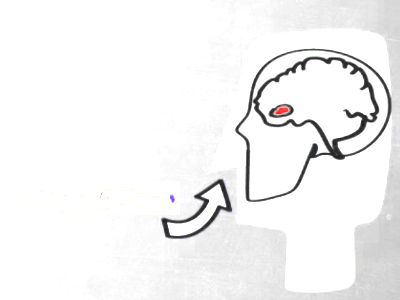
\includegraphics[height=0.5\textheight]{motivazioni/intro_1.png}
\end{column}
\begin{column}{0.5\textwidth}
\only<1>{
\begin{quote}
    how can we build tiny little robots that are able to enter the human body through natural orifices or small incisions, to reach places minimally invasively for surgery?
    \begin{flushright}
    \tiny{---Jessica Burgner-Kahrs}
    \end{flushright}
\end{quote}
}
\only<2>{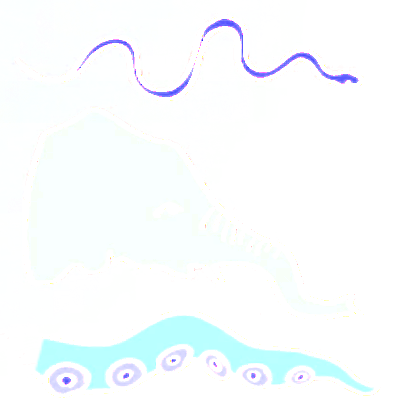
\includegraphics[height=0.5\textheight]{motivazioni/intro_2.png}}
\end{column}
\end{columns}
\Reference{Task-specific Design of Tubular Continuum Robots for Surgical Applications}{Burgner-Kahrs}{2015}

\note{
Manipolatori che entrano nel corpo per operare in modo minimamente invasivo. \\

Robot continui, ispirati alle forme presenti in natura.\\

Struttura capace di piegarsi in ogni punto. \\
}

\end{frame}


\begin{frame}{Obiettivi}
    \begin{itemize}
        \item<1-> caratteristiche dei manipolatori continui
        \item<2-> utilizzi in campo medico
        \item<3-> modellazione del robot
        \item<4-> confronto di tecniche per la cinematica inversa
    \end{itemize}
    
\note{
Quattro obiettivi principali (in elenco). 
}
\end{frame}

\TransitionFrame{caratteristiche dei manipolatori continui}

\begin{frame}{Terminologia}
\begin{columns}
\begin{column}{0.5\textwidth}
\begin{itemize}
    \item<1-> \textcolor{yellow}{continuum robot}
    \item<2-> hyperredundant robot
    \item<3-> pseudocontinuum robot
\end{itemize}
\end{column}
\begin{column}{0.5\textwidth}
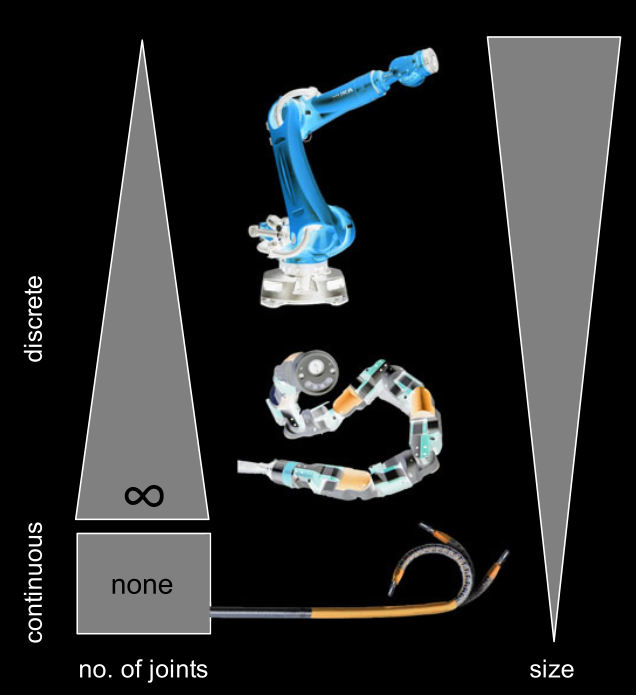
\includegraphics[width=\textwidth]{slide_studio/img_terminologia/terminologia.png}
\end{column}
\end{columns}

\BReference{Continuum Robots for Medical Application: A Survey}{Burgner-Kars, Rucker}{2015}

\note{
Continuum robot $\to$ struttura attuabile il cui materiale costitutivo forma una curva differenziabile. Definizioni alternative: $\infty$-DOF, senza link rigidi, senza giunti identificabili. \\

Hyperredundant robot $\to$ numero elevato di link e giunti. Il materiale costitutivo forma una linea spezzata che approssima una curva differenziabile con precisione arbitraria. \\

Pseudo-continuum robot $\to$ sia link rigidi che elementi in grado di piegarsi in modo continuo.
}
\end{frame}


\begin{frame}{Struttura}
\begin{columns}
\begin{column}{0.5\textwidth}
\begin{itemize}
    \item<1-> single backbone
    \item<2-> multi-backbone
    \item<3-> a tubi concentrici
\end{itemize}
\end{column}
\begin{column}{0.5\textwidth}
\only<1>{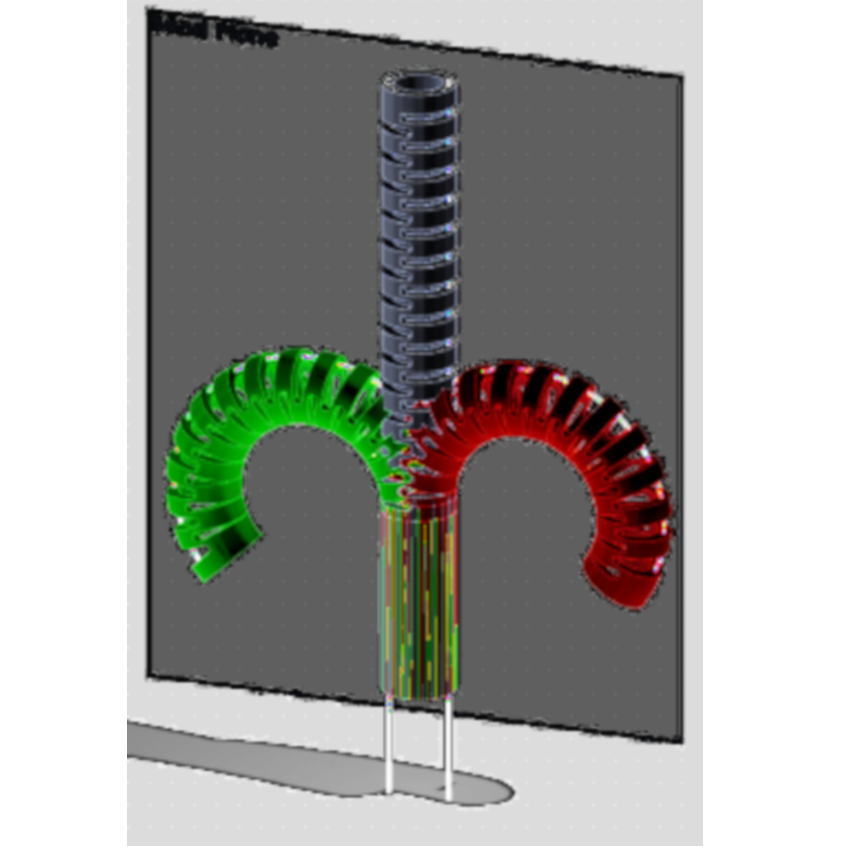
\includegraphics[height=0.7\textheight]{slide_studio/img_struttura/single_backbone.png}}
\only<2>{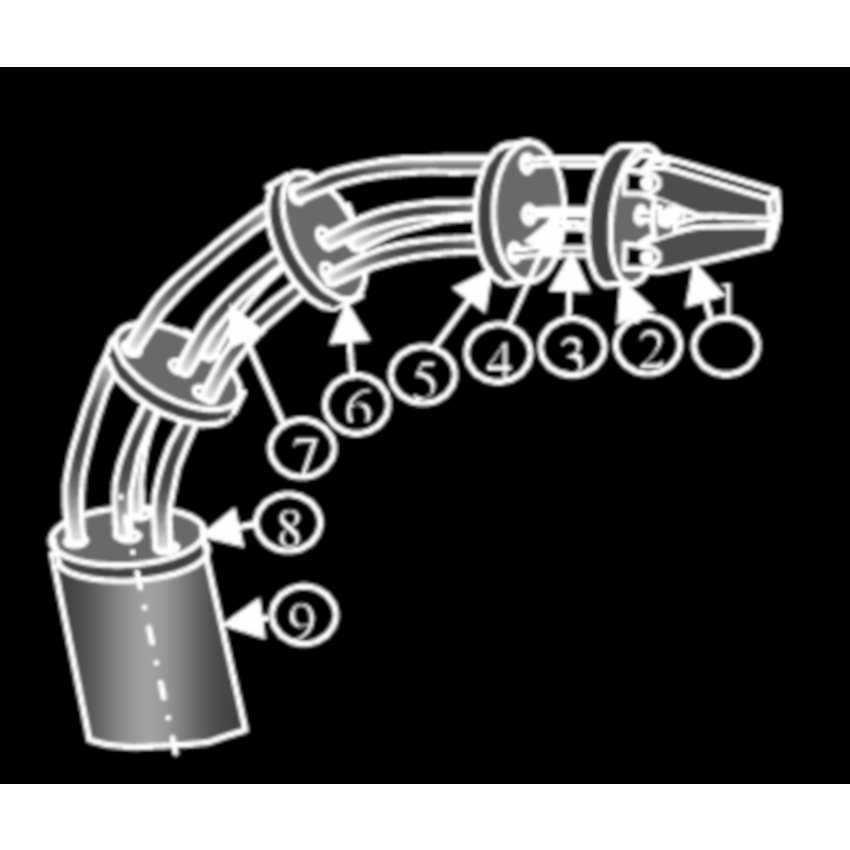
\includegraphics[height=0.7\textheight]{slide_studio/img_struttura/multi_backbone.png}}
\only<3>{\hspace*{-4em}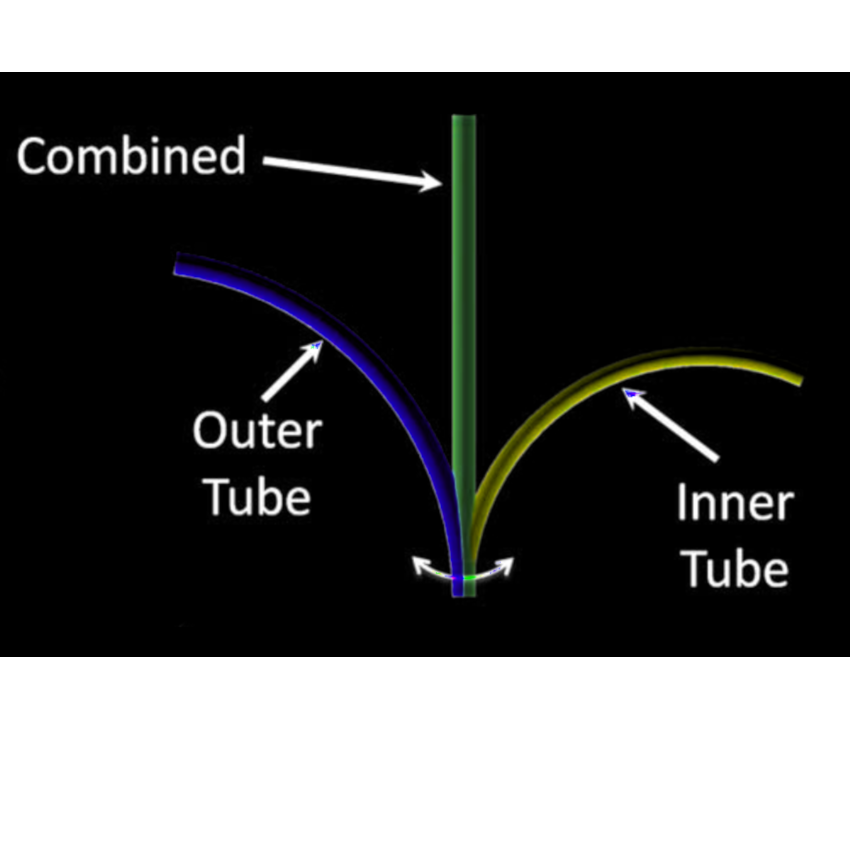
\includegraphics[height=0.7\textheight]{slide_studio/img_struttura/tubi_concentrici.png}}
\end{column}
\end{columns}

\only<1>{\Reference{Design of a new cable-driven manipulator with a large open lumen: Preliminary applications in the minimally-invasive removal of osteolysis}{Kutzer et al.}{2011}}

\only<2>{\Reference{Snake-Like Units Using Flexible Backbones and Actuation Redundancy for Enhanced Miniaturization}{Kutzer et al.}{2011}}

\only<3>{\BReference{Design and Control of Concentric-Tube Robots}{Dupont et al.}{2010}}

\note{
Single backbone $\to$ struttura elastica centrale, fa passare trasmissione, attuazione e strumenti.

Multi-backbone $\to$ elementi elastici paralleli ma vincolati. [Spiega figura: tirando 2 su 3 backbone secondarie, muovi il manipolatore in ogni direzione].

Tubi concentrici $\to$ tubi pre-curvati uno dentro l'altro. La base di ognuno viene ruotata e traslata assialmente per controllare la forma del robot. 
}
\end{frame}

\begin{frame}{Struttura}
\begin{columns}
\begin{column}{0.5\textwidth}
Solitamente composto da due componenti separate:
\begin{itemize}
    \item<2-> parte prossimale 
    \item<3-> parte distale
\end{itemize}
\end{column}
\begin{column}{0.5\textwidth}
{\centering 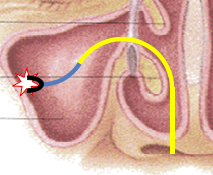
\includegraphics[height=0.5\textheight]{slide_studio/img_struttura/distal_proximal.png}}
\end{column}
\end{columns}

\note{
Può essere diviso in parte prossimale (raggiunge luogo operazione) e distale (effettua operazione).
}

\end{frame}
\begin{frame}{Attuazione}
\begin{columns}

\column{0.5\textwidth}
\begin{itemize}
    \item<1-> estrinseca
    \begin{itemize}
        \item <3-> nelle strutture multi-backbone
        \item <4-> nelle strutture a tubi concentrici
    \end{itemize}
    \item<2-> intrinseca
    \begin{itemize}
        \item<5-> attraverso camera idraulica
        \item<6-> attraverso shape memory effect
        \item<7-> attraverso micro-motori
        \item<8-> attraverso campi magnetici generati da MRI
    \end{itemize}
\end{itemize}

\column{0.5\textwidth}
\only<1-2>{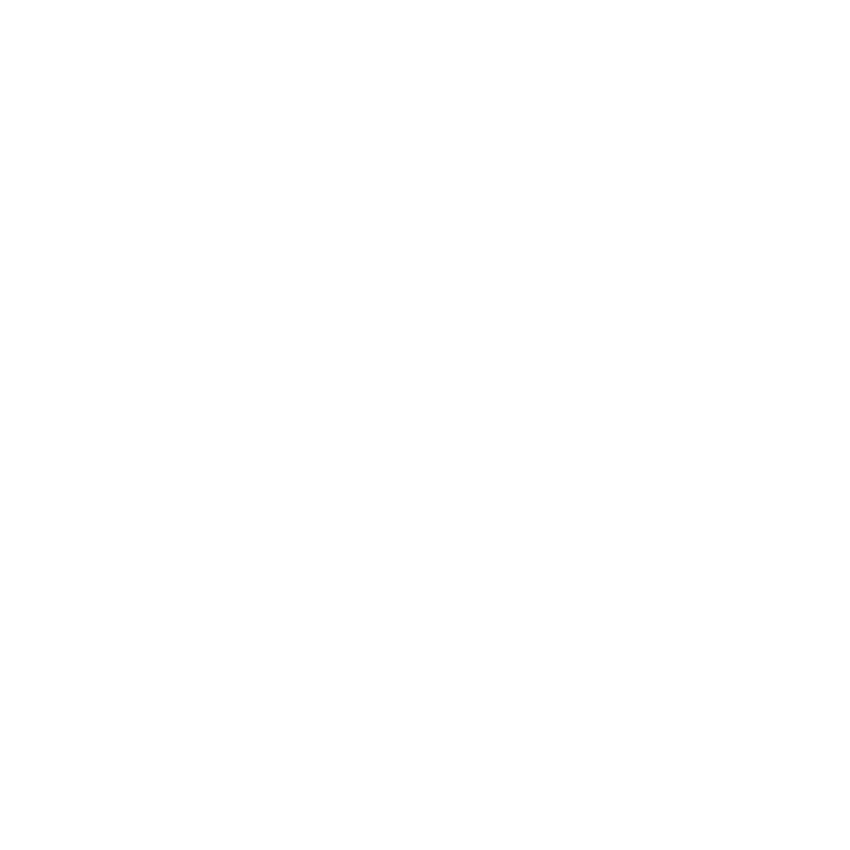
\includegraphics[height=0.7\textheight]{slide_studio/img_attuazione/attuazione_none.png}}
\only<3>{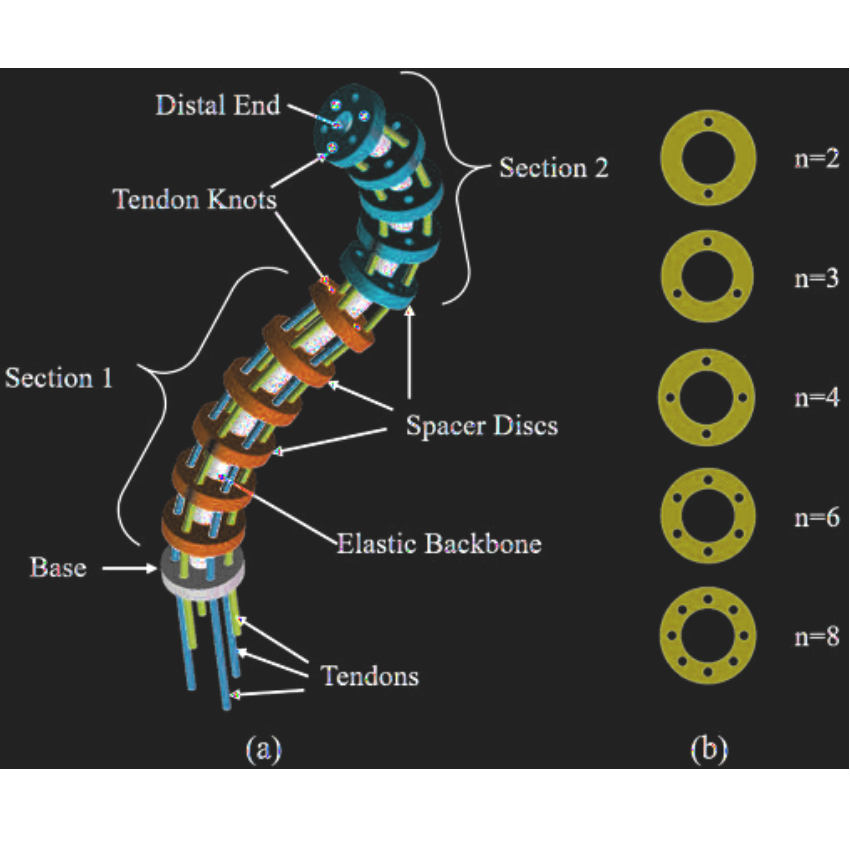
\includegraphics[height=0.7\textheight]{slide_studio/img_attuazione/attuazione_ext_multibackbone.png}}
\only<4>{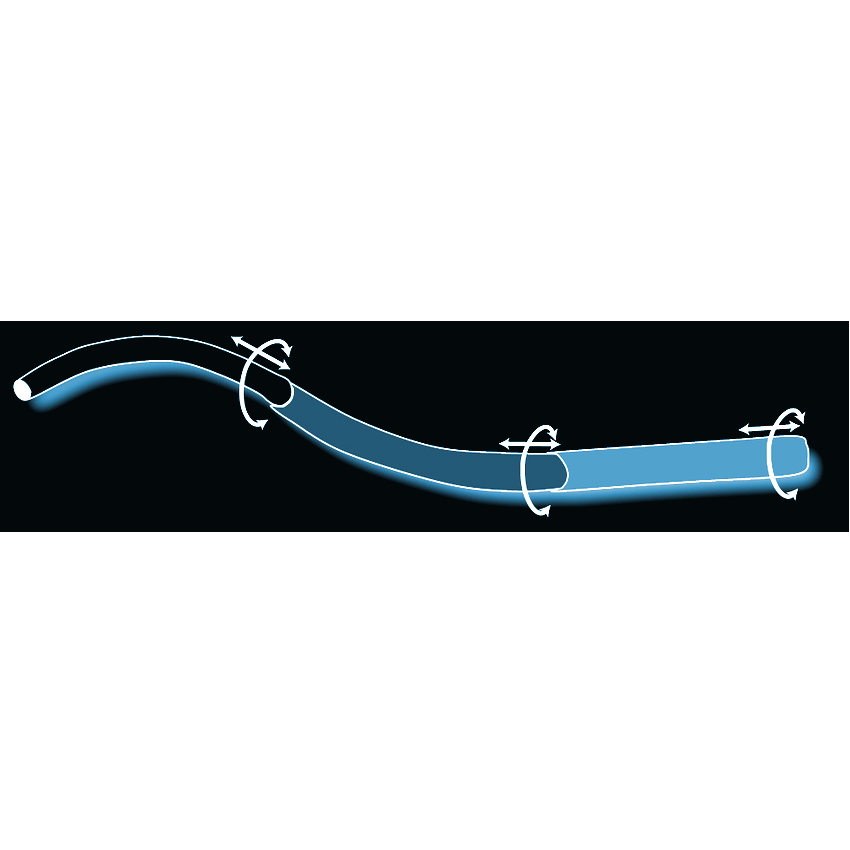
\includegraphics[height=0.7\textheight]{slide_studio/img_attuazione/attuazione_ext_concentrico.png}}
\only<5>{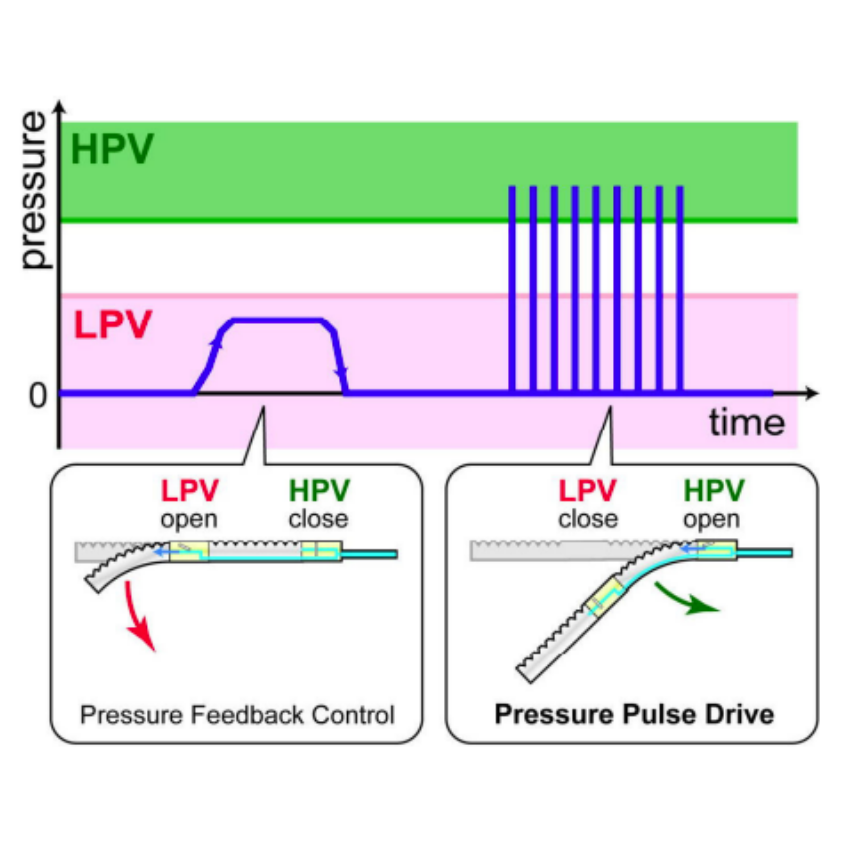
\includegraphics[height=0.7\textheight]{slide_studio/img_attuazione/attuazione_int_valvole.png}}
\only<6>{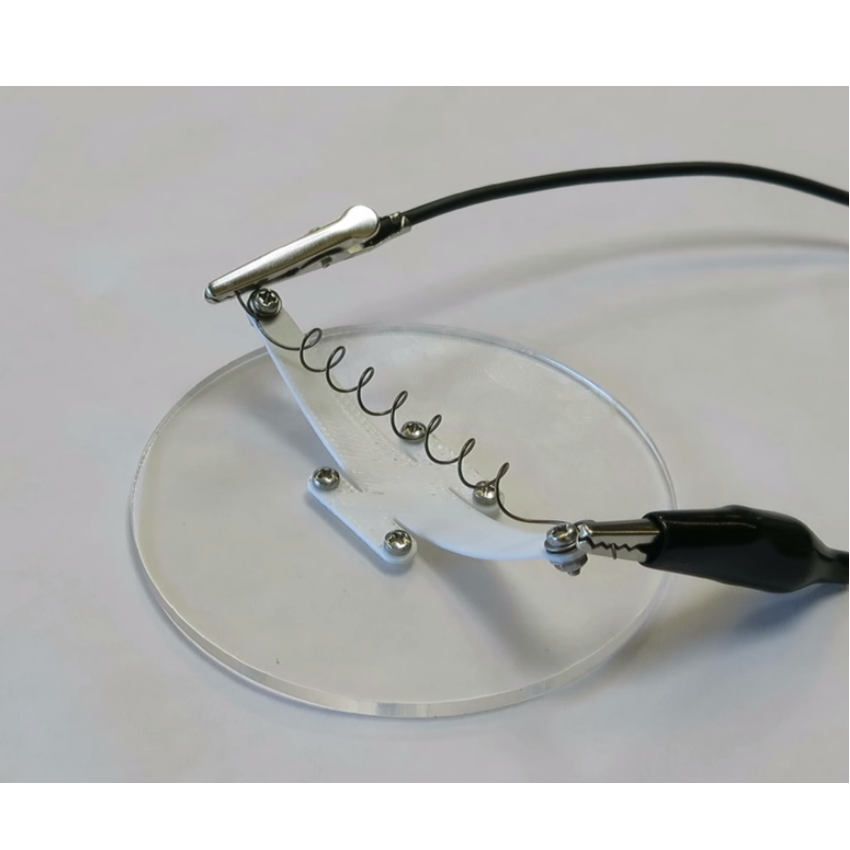
\includegraphics[height=0.7\textheight]{slide_studio/img_attuazione/attuazione_int_shapememory.png}}
\only<7>{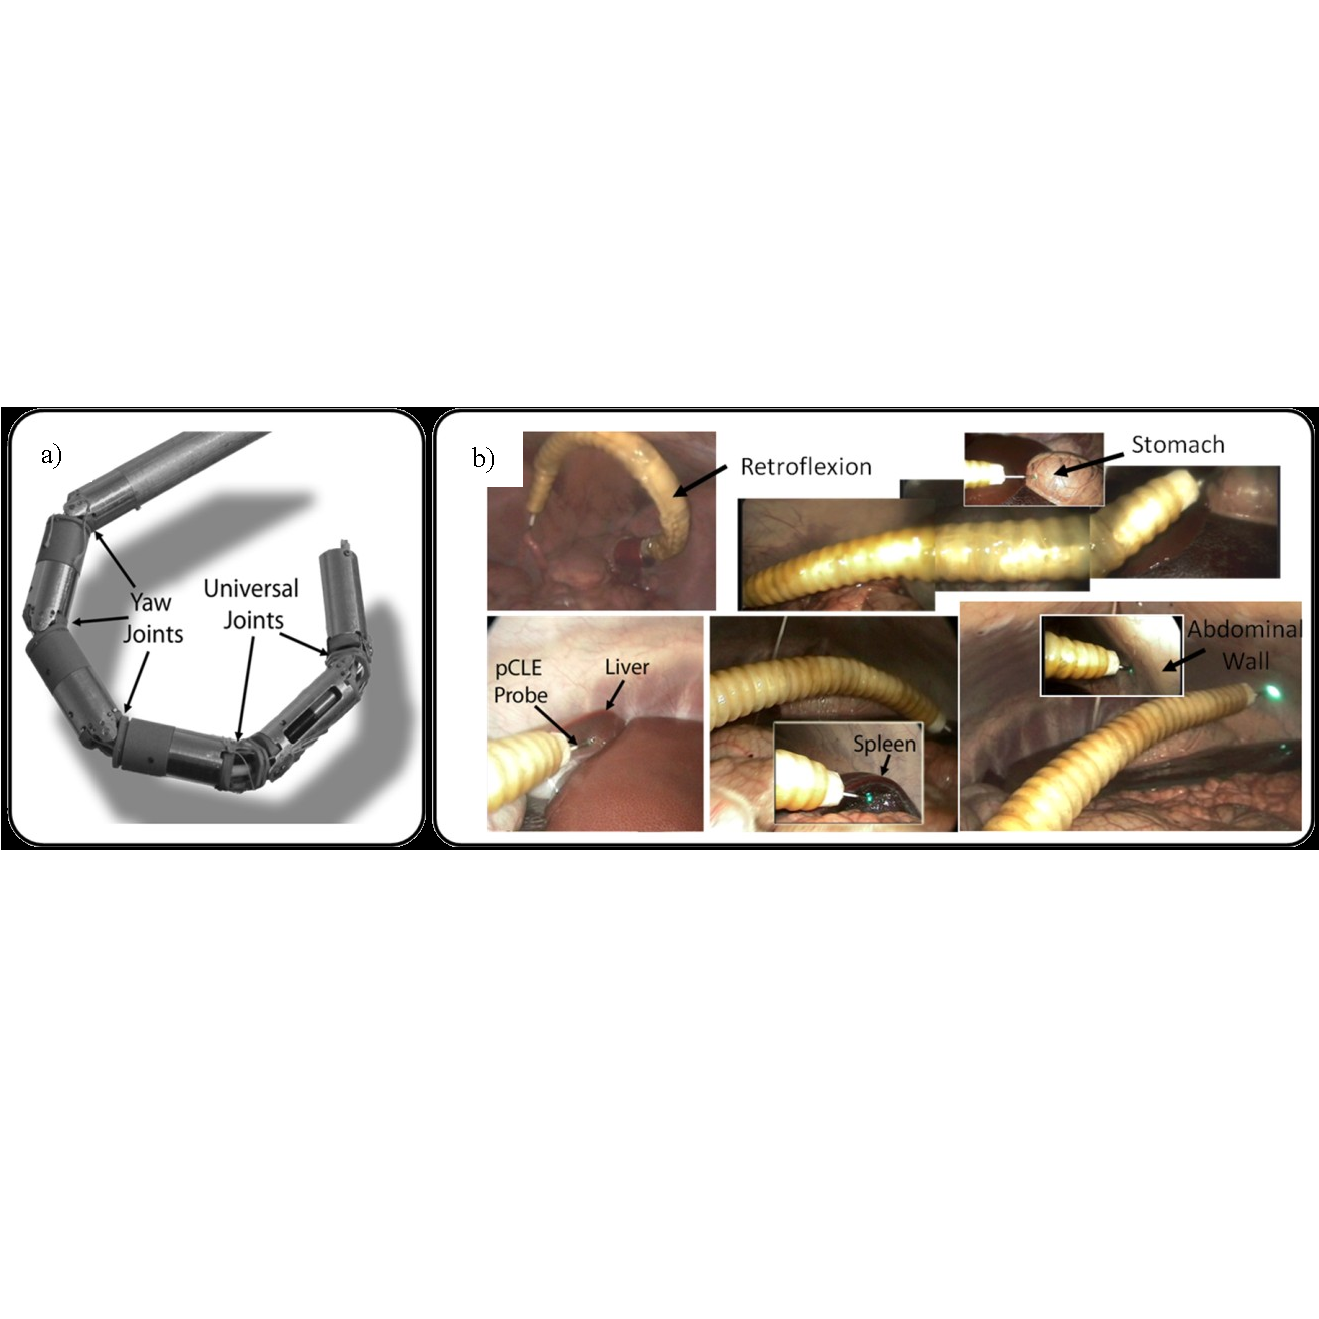
\includegraphics[height=0.7\textheight]{slide_studio/img_attuazione/attuazione_int_motori.png}}
\only<8>{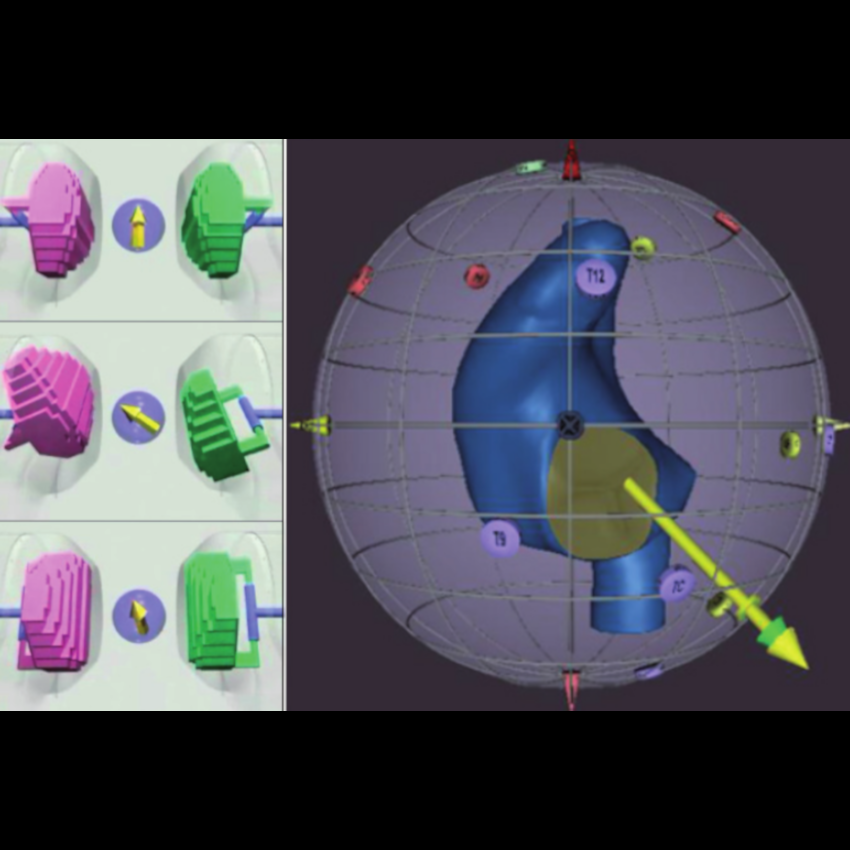
\includegraphics[height=0.7\textheight]{slide_studio/img_attuazione/attuazione_int_mri.png}}

\end{columns}

\only<3>{\Reference{Kinematic comparison of surgical tendon-driven manipulators and concentric tube manipulators}{Li, Wu, Ren, You}{2017}}
\only<4>{\Reference{Workspace characterization for concentric tube continuum robots}{Burgner-Kahrs et al.}{2014}}
\only<5>{\Reference{Precise Bending Angle Control of Hydraulic Active Catheter by Pressure Pulse Drive}{Ikuta et al.}{2010}}
\only<6>{\Reference{Clip ``SMA actuator design"}{\url{https://www.youtube.com/watch?v=PxBPpPRkv6A}}{2015}}
\only<7>{\Reference{A modular, mechatronic joint design for a flexible access platform for MIS}{Noonan et al.}{2011}}
\only<8>{\Reference{Stereotaxis Niobe magnetic navigation system for endocardial catheter ablation and gastrointestinal capsule endoscopy}{Carpi, Pappone}{2009}}

\note{
Attuazione $\to$ punto in cui la potenza viene convertita in energia meccanica. 

Estrinseca $\to$ fuori dalla struttura (diametro robot minore). 

Intrinseca $\to$ dentro la struttura (minore frizione, minore footprint in sala operatoria).

Estrinseca multibackbone $\to$ tendini, cavi da tirare per dare la curvatura desiderata. 

Estrinseca tubi concentrici $\to$ ruoto e traslo base dei tubi per controllare forma del robot. 
Intrinseco idrulico $\to$ valvole che si aprono ad uno specifico range di pressione (driving range). Il liquido confluisce in una o l'altra direzione, muovendo il manipolatore. 

Intrinseco shape memory $\to$ proprietà delle leghe metalliche. Il materiale si deforma sottoposto ad un carico, torna alla forma originale se riscaldato. 

Intrinseco micro-motori $\to$ devono essere piccoli. 

Intrinseco MRI $\to$ usato nei cateteri con punta magnetica. Viene mosso da campo magnetico generato da una macchina simile allo scanner MRI.
}
\end{frame}

\begin{frame}{Cinematica}
\begin{columns}
\begin{column}{0.5\textwidth}
\begin{itemize}
    \item<1-> \textcolor{yellow}{rigid link}
    \item<2-> \textcolor{yellow}{piecewise constant curvature}
    \item<3-> piecewise variable curvature
\end{itemize}
\end{column}
\begin{column}{0.8\textwidth}
\only<1>{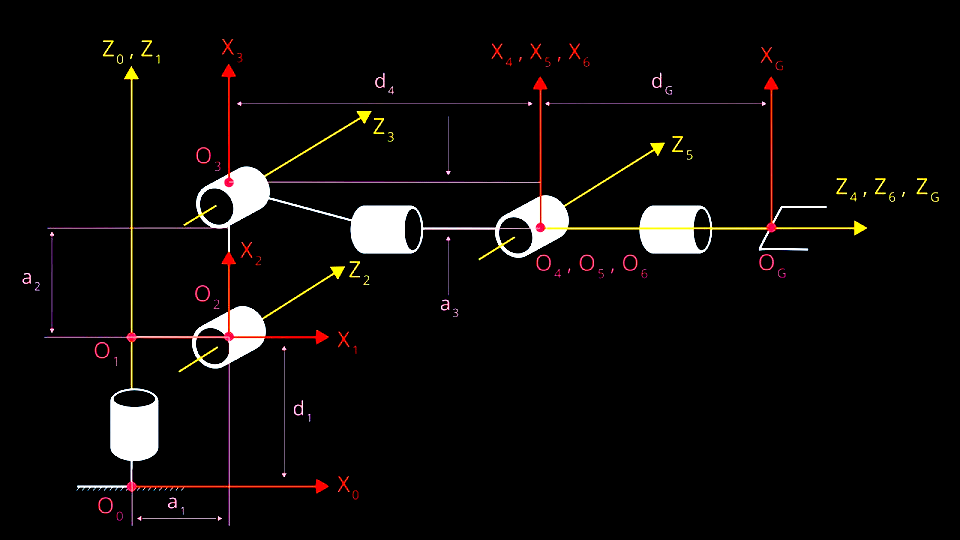
\includegraphics[height=0.7\textheight, trim={0 0 2cm 0},clip]{slide_studio/img_cinematica/kinematics_dh.png}}
\only<2>{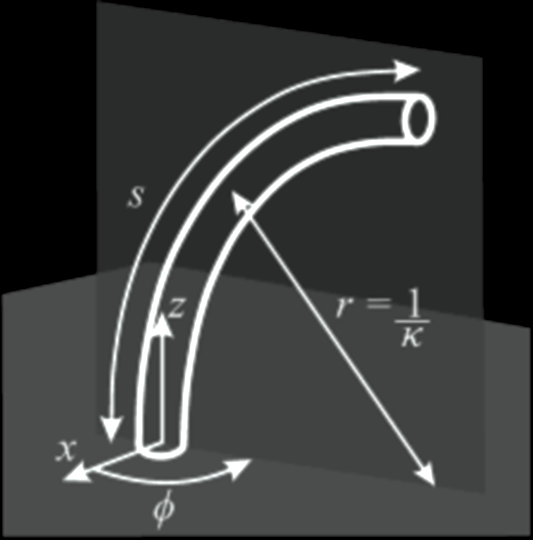
\includegraphics[height=0.7\textheight]{slide_studio/img_cinematica/kinematics_constant_curvature.png}}
\only<3>{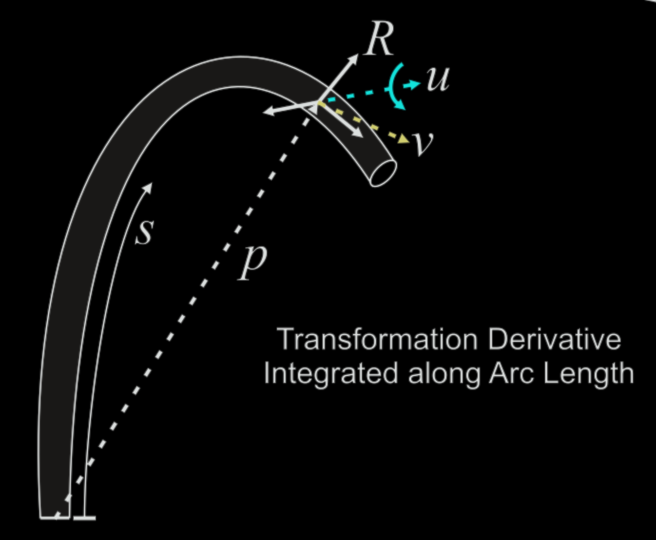
\includegraphics[height=0.7\textheight]{slide_studio/img_cinematica/kinematics_variable_curvature.png}}
\end{column}
\end{columns}
\only<1>{\Reference{Inverse Kinematics on Kuka Arm using ROS and Python}{\url{https://nitishpuri.github.io/posts/robotics/inverse-kinematics-on-kuka-arm-using-ros-and-python/}}{2019}}
\only<2>{\Reference{Design and Kinematic Modeling of Constant Curvature Continuum Robots: A Review}{Webster, Jones}{2010}}
\only<3>{\Reference{A variable curvature continuum kinematics for kinematic control of the bionic handling assistant}{Mahl et al.}{2014}}

\note{
Modello a link rigidi $\to$ link e giunti rotatori e prismatici. Posizione end-effector è funzione dei valori (di angolo, di distanza) del giunto. 

Modello piecewise constant curvature $\to$ segmenti o pezzi, ogni pezzo ha curvatura costante su tutta la lunghezza dell'arco. Posizione è funzione di rotazione e curvatura del segmento. 

Modello piecewise variable curvature $\to$ rimuovo vincolo curvatura costante per tutto il segmento. 
}
\end{frame}
\TransitionFrame{utilizzi in campo medico}

\begin{frame}{Alcune applicazioni in campo medico}
\begin{columns}
\begin{column}{0.5\textwidth}
\begin{itemize}
    \item<1-> neurochirurgia
    \begin{itemize}
        \item<2-> somministrazione intracerebrale di farmaci
        \item<3-> rimozione di emorragie
    \end{itemize}
    \item<4-> otorinolaringoiatria
    \begin{itemize}
        \item<5-> Functional Endoscopic Sinus Surgery
        %\item<6-> chirurgia della gola
    \end{itemize}
    \item<6-> cardiochirurgia
    \begin{itemize}
        \item<6-> chirurgia intracardiaca per via percutanea
    \end{itemize}
    %\item<7-> chirurgia vascolare
    \item<7-> ...
\end{itemize}
\end{column}
\begin{column}{0.8\textwidth}
\only<1>{\hspace*{1em}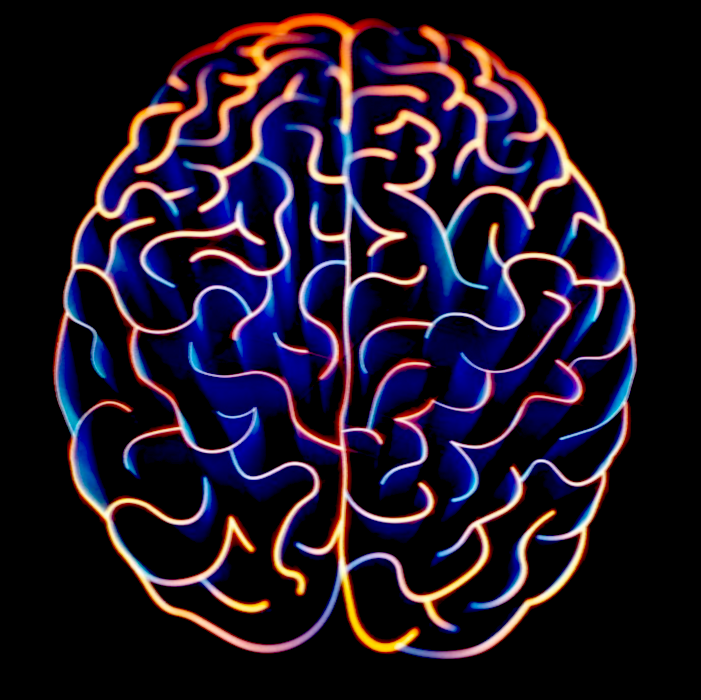
\includegraphics[height=0.7\textheight]{slide_uso/uso_neuro.png}}
\only<2>{\hspace*{1em}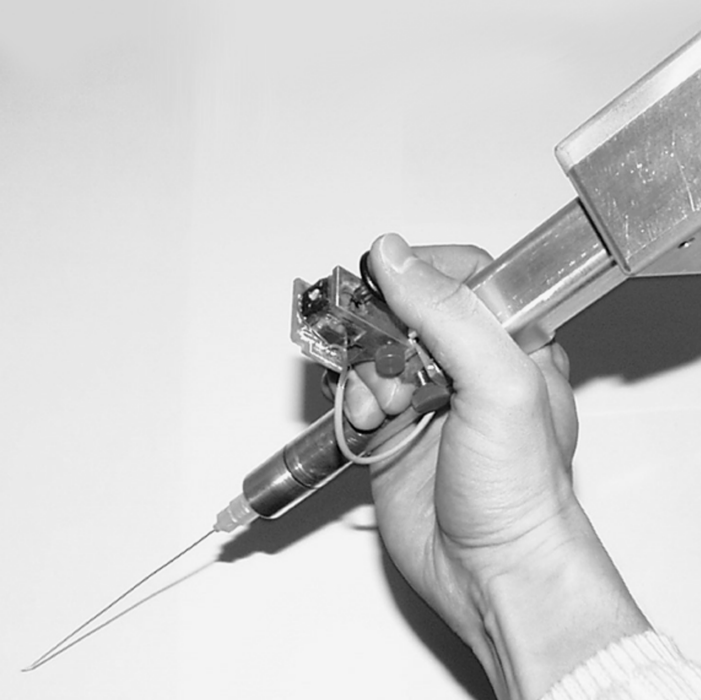
\includegraphics[height=0.7\textheight]{slide_uso/uso_neuro_drugdelivery.png}}
\only<3>{\hspace*{1em}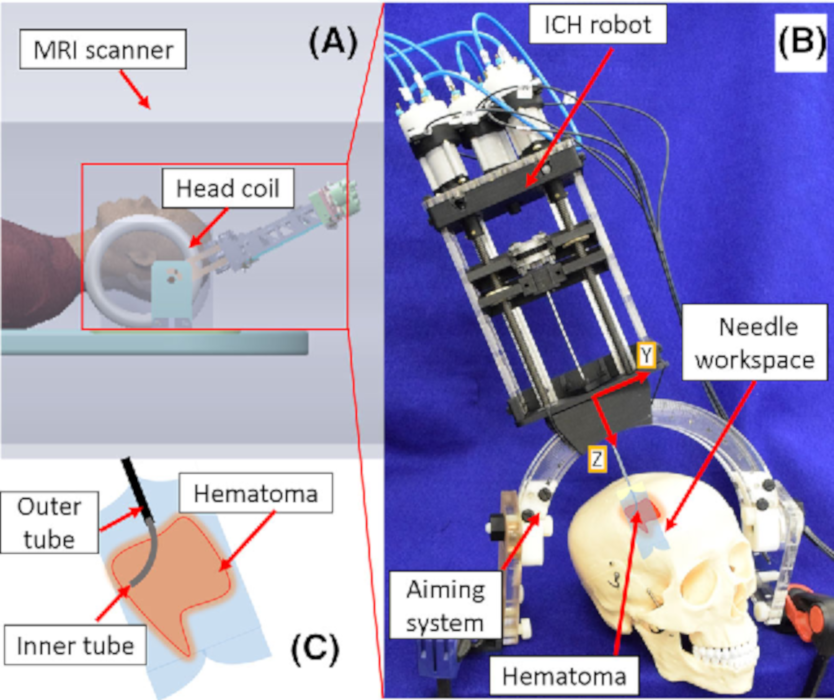
\includegraphics[height=0.7\textheight]{slide_uso/uso_neuro_hematoma.png}}
\only<4>{\hspace*{1em}
\includegraphics[height=0.7\textheight]{slide_uso/usi_otorinolaringoiatria.png}}
\only<5>{\hspace*{1em}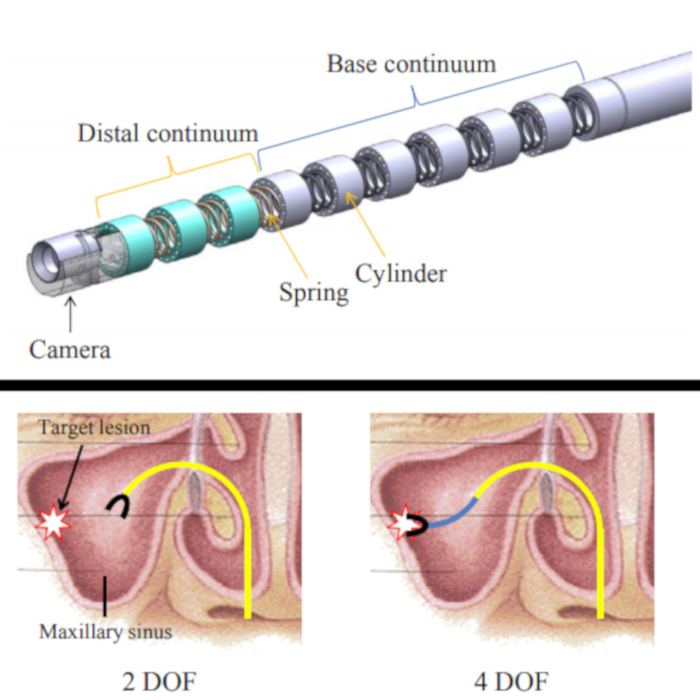
\includegraphics[height=0.7\textheight]{slide_uso/uso_otorino_fess.png}}
%\only<6>{\hspace*{1em}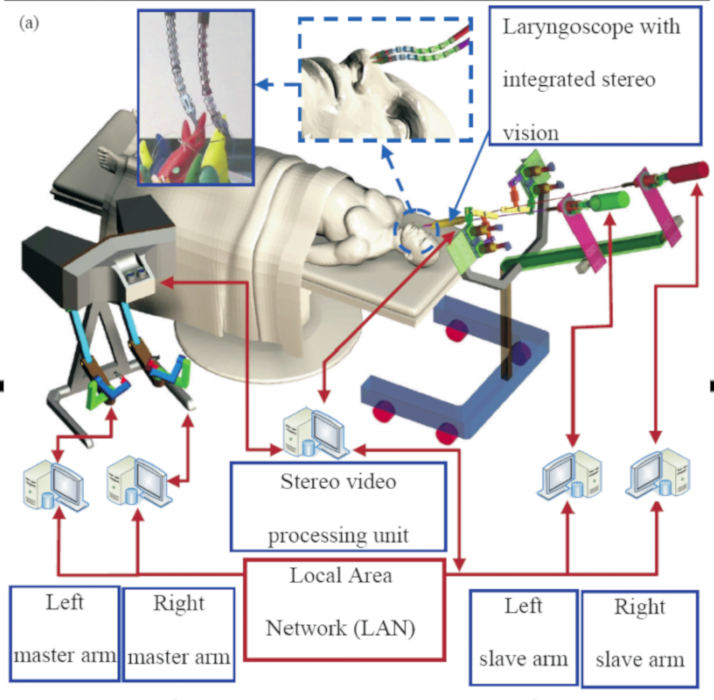
\includegraphics[height=0.7\textheight]{slide_uso/uso_otorino_throat.png}}
\only<6>{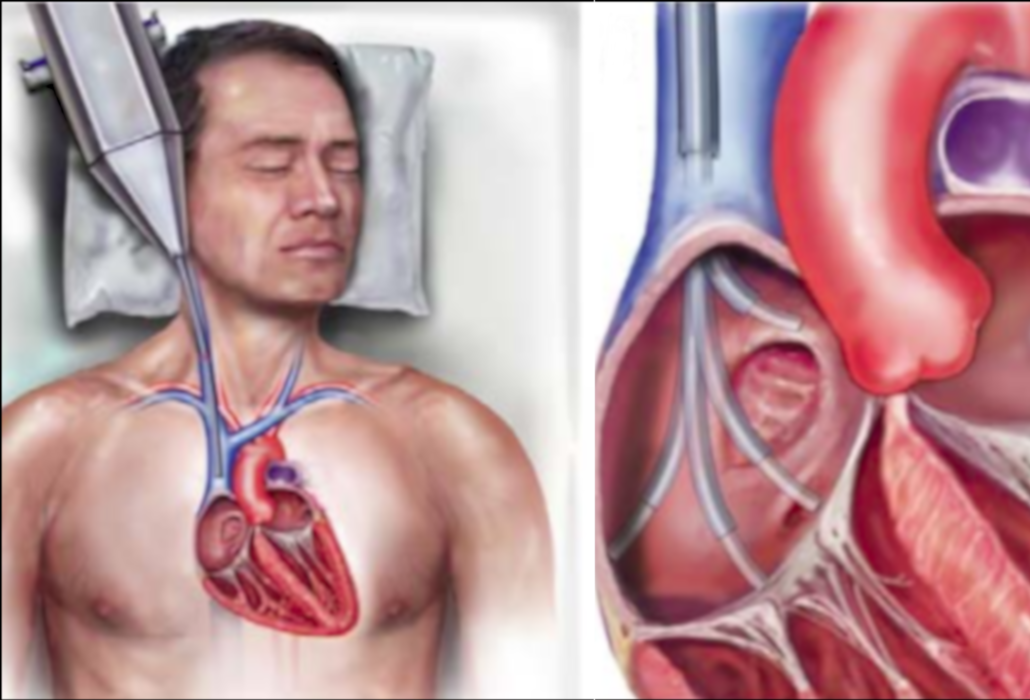
\includegraphics[height=0.7\textheight]{slide_uso/uso_cardio.png}}
\only<7>{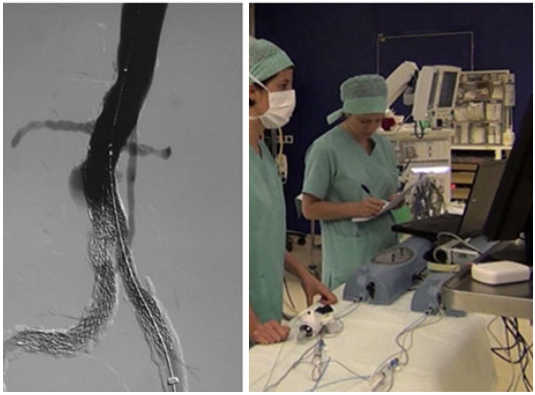
\includegraphics[height=0.7\textheight]{slide_uso/uso_vascolare.png}}
\end{column}
\end{columns}
\only<2>{\Reference{Design choices in needle steering: A review}{Van der Berg et al.}{2015}}
\only<3>{\Reference{Debulking From Within: A Robotic Steerable Cannula for Intracerebral Hemorrhage Evacuation}{Burgner et al.}{2013}}
\only<5>{\Reference{Compact Design of a Dual Master-Slave System for Maxillary Sinus Surgery}{Yoon et al.}{2013}}
%\only<6>{\Reference{Design and Integration of a Telerobotic System for Minimally Invasive Surgery of the Throat}{Simaan, Xu, Wei}{2009}}
\only<6>{\Reference{Percutaneous Steerable Robotic Tool Delivery Platform and Metal Microelectromechanical Systems Device for Tissue Manipulation and Approximation}{Vasiyev et al.}{2013}}
%\only<7>{\Reference{Current and Emerging Robot-Assisted Endovascular Catheterization Technologies: A Review}{Rafii-Tari, Payne, Yang}{2013}}

\note{
Neurochirurgia rischi $\to$ grandi aperture, spostamento dei tessuti per raggiungere regioni più profonde. 

Neurochirurgia: somministrazione intracerebrale farmaci $\to$ manipolatori tip steereble needle (punta orientabile) portano l'ago nell'esatta posizione, possono essere costrutiti tramite tubi concentrici. 

Neurochirurgia: rimozione emorragie $\to$ manipolatore a (due) tubi concentrici. Quello esterno diritto raggiunge il luogo. Quello interno, curvo, è interscambiabile per raggiunge coaguli di forme e dimensioni diverse.

Otorino-laringo-iatria $\to$ (zona orecchie naso gola) Parte superiore ed inferiore seno mascellare difficili da raggiungere.  Endoscopio 4 gdl (2+2 prossimale+distale) supera le limitazioni di quello classico diritto. 

Cardiochirurgia rischi $\to$ operazioni a cuore aperto, operazioni senza battito. 
Proposta di operazione al cuore $\to$ attraverso catetere = manipolatore composto da parte prossimale per raggiungere il luogo e distale per manipolare i tessuti, implementato tramite tubi concentrici per il loro diametro ridotto.
}
\end{frame}
\TransitionFrame{modellazione del robot}

\begin{frame}{Modellazione}
\begin{columns}

\begin{column}{0.5\textwidth}
\begin{itemize}
    \item<1-> modello \textcolor{yellow}{discreto}
    \begin{itemize}
        \item<2-> approssimano un manipolatore continuo
    \end{itemize}
    \item<3-> numero $T$ arbitrario di link rigidi
    \item<4-> ogni link ha lunghezza $\ell_i$
    \begin{itemize}
        \item<5-> $N$ link con lunghezza $\ell_i$ grande per la parte prossimale
        \item<6-> $M$ link con lunghezza $\ell_j < \ell_i$ per la parte distale
        \item<6-> $T=N+M$
    \end{itemize}
    \item<7-> ogni giunto è sferico
    \begin{itemize}
        \item<8-> due giunti separati
        \item<9-> uno ruota sul proprio asse $x$
        \item<10-> uno ruota sul proprio asse $y$
    \end{itemize}
\end{itemize}
\end{column}

\begin{column}{0.6\textwidth}
\begin{center}
\only<1-6>{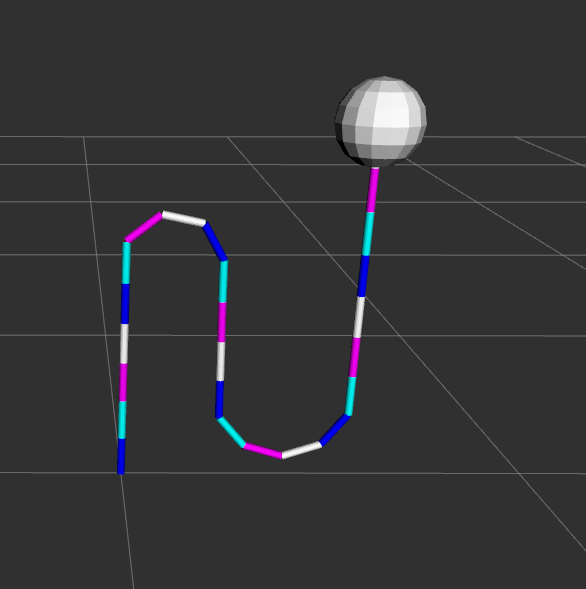
\includegraphics[height=0.7\textheight]{slide/img_modellazione/manipolatore-32-48.png}}
\only<7-10>{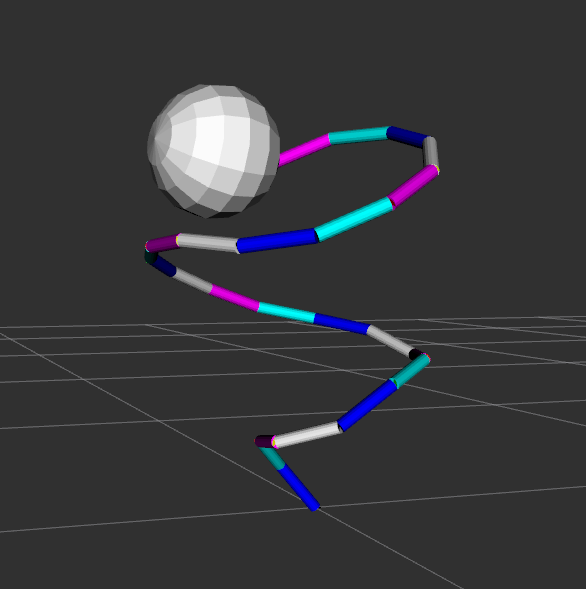
\includegraphics[height=0.7\textheight]{slide/img_modellazione/manipolatore-29-36.png}}
\end{center}
\end{column}
\end{columns}

\note{
Parte pratica \# 1: proporre modellazione manipolatori. 

Utilizzo modello rigid link, numero discreto di segmenti rigidi approssima con precisione arbitraria ogni manipolatore continuo. 

La lunghezza di ogni link non è necessariamente uguale $\to$ parte distale e prossimale.

Il giunto tra due link è sferico, viene modellato attraverso due giunti separati, uno che ruota intorno l'asse x ed uno intorno ad $y$. 
}

\end{frame}


\begin{frame}{Spazio di raggiungibilità}
\begin{columns}
\begin{column}{0.5\textwidth}
\begin{itemize}
    \item<1-> calcolo dello spazio di raggiungibilità
    \begin{itemize}
        \item<2-> semisfera
        \item<3-> raggio $r = \sum_{i = 1}^n \ell_i$
    \end{itemize}
\end{itemize}
\end{column}
\begin{column}{0.8\textwidth}
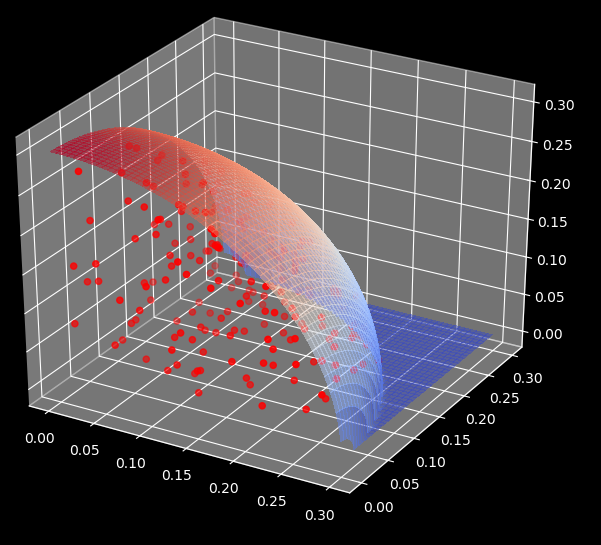
\includegraphics[width=0.7\textwidth]{slide/img_modellazione/spazio_raggiungibilita_red.png}
\end{column}
\end{columns}

\note{
Lo spazio di raggiungibilità del manipolatore è una semisfera di raggio pari alla somma delle lunghezze dei segmenti. 

L'end-effector deve essere quindi in grado di raggiungere i punti rossi del grafico. 
}

\end{frame}
\TransitionFrame{confronto di tecniche per la cinematica inversa}

\begin{frame}{Framework}

% loghi
\begin{columns}
\begin{column}{0.5\textwidth}
\begin{center} TRAC-IK\end{center}
\begin{center}
    
\includegraphics[width=0.2\textwidth]{slide/img_cinematica_inversa/trac-ik.png}
\end{center}
\end{column}
\begin{column}{0.5\textwidth}
\begin{center} SCIPY\end{center}
\begin{center}
    
\includegraphics[width=0.4\textwidth]{slide/img_cinematica_inversa/scipy.png}
\end{center}
\end{column}
\end{columns}

% descrizione
\begin{columns}
\begin{column}{0.5\textwidth}
\begin{itemize}
    \item<1-> ottimizzazione applicata alla cinematica inversa
    \item<4-> package del framework ROS
    \item<6-> Newton + SLSQP
\end{itemize}
\end{column}
\begin{column}{0.5\textwidth}
\begin{itemize}
    \item<2-> ottimizzazione ``general purpose"
    \begin{itemize}
        \item<3-> flessibile
    \end{itemize}
    \item<5-> libreria di Python
    \item<7-> diversi algoritmi
    \begin{itemize}
        \item<7-> L-BFGS-B, TNC, SLSQP, COBYLA
    \end{itemize}
\end{itemize}
\end{column}
\end{columns}

% references
\btVFill

\only<1>{\footnotesize \emph{TRAC-IK: An open-source library for improved solving of generic inverse kinematics}, Beeson, Ames, 2015}
\only<2>{\footnotesize \emph{SciPy 1.0: fundamental algorithms for scientific computing in Python}, Virtanen et al., 2020}

\note{
Specchietto cinematica inversa $\to$ mapping da spazio di raggiungibilità a spazio dei giunti. Soluzione non garantita esistere, non garantita unica (ridondanza). Analitica/forma chiusa vs numerica/iterativa. Numerica $\to$ usa Jacobiano analitico (differenzio funzione cinenmatica rispetto al tempo). Devo evitare singolarità (J perde rango) = l'end effector non può muoversi in una direzione. Vicino singolarità = piccoli spost endeffector diventano grandi spostamenti variabili di giunto. 

Parte pratica \# 2 $\to$ tecniche per la realizzazione della cinematica inversa. Proposti due software.

primo: TRAC-IK $\to$ il migliore dei pacchetti per la cinemativa inversa in ROS.

secondo: script $\to$ modella cinematica inversa come problema di ottimizzazione che viene dato in input a SCIPY, libreria di ottimizzazione per python. Più flessibile: funzione di costo può essere arricchita per valutare altri aspetti es. forma.  

Distribuzione $\to$ pkg ROS vs sorgente python 3.0. 

Algoritmo TRAC-IK $\to$ esecuzione concorrente di due, uno basato su Newton e l'altro su Quasi-Newton. Newton converge velocemente ma richiede calcolo hessiana ed inversione ad ogni step. Quasi-Newton approssima hessiana aggiornata usando il gradiente calcolato nel punto, ad ogni iterazione, l'hessiana è stimata già invertita. Più lenta convergenza. L'algoritmo è Sequential Least Square Quadratic Programming. 

Algoritmo script $\to$ tutti quelli messi a disposizione da SCIPY. 
}
\end{frame}













\begin{frame}{Formalizzazione dei problemi}
\begin{columns}
\begin{column}{0.5\textwidth}
\begin{itemize}
    \item<1-> generazione punti end-effector \textcolor{red}{$\bullet$}
    \item<2-> primo problema:
    \begin{itemize}
        \item<3-> input: \textcolor{red}{$\bullet$}
        \item<4-> output: configurazione che fa coincidere la posizione dell'end-effector con \textcolor{red}{$\bullet$}
    \end{itemize}
    \item<5-> generazione punti intermedi  \textcolor{blue}{$\bullet$}
    \item<6-> secondo problema:
    \begin{itemize}
        \item<7-> input: \textcolor{red}{$\bullet$}, \textcolor{blue}{$\bullet$}
        \item<8-> output: configurazione che fa coincidere la posizione dell'end-effector con \textcolor{red}{$\bullet$} minimizzando la distanza del manipolatore da \textcolor{blue}{$\bullet$}
    \end{itemize}
\end{itemize}
\end{column}
\begin{column}{0.8\textwidth}
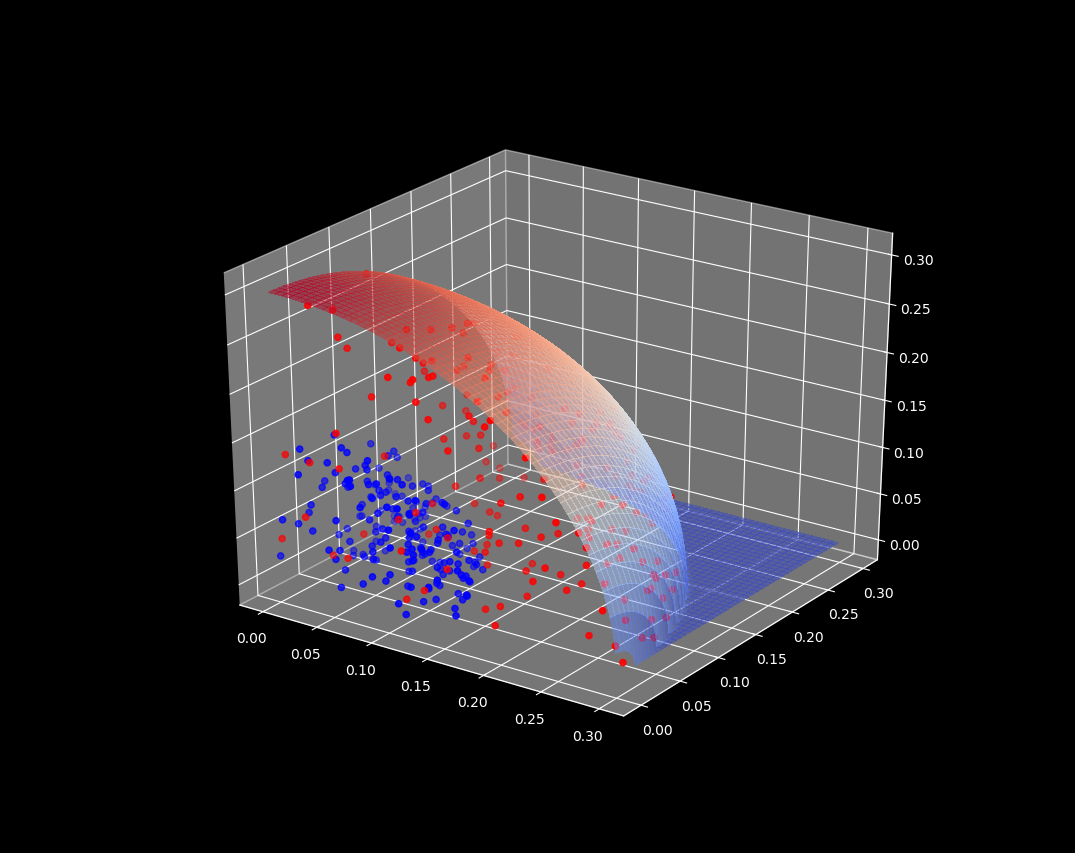
\includegraphics[height=0.9\textheight,trim={0 0 0cm 0},clip]{slide/img_cinematica_inversa/spazio_raggiungibilita.png}
\end{column}
\end{columns}

\note{
Testo validità dei due approcci. Due problemi. 

\# 1 $\to$ problema cinematico inverso puro.

\# 2 $\to$ problema cinematico inverso che cerca di imporre una data forma al manipolatore
}
\end{frame}










\begin{frame}{Ottimizzazione}

    \begin{itemize}
        \item<1->[] Definiamo $\mathrm{directkin}(\vec{\theta})$ la funzione di cinematica diretta del manipolatore.
        \item<2->[] Definiamo $\mathrm{d}(p_1, p_2)$ la distanza tra due punti, $\mathrm{d}_\text{man}(p, \vec{\theta})$ la distanza di un punto $p$ dal manipolatore nella configurazione $\vec{\theta}$.
        \item<3->[] \[ \text{problema1}(\textcolor{red}{\bullet}) = \argmin\limits_{\vec{\theta}} d(\textcolor{red}{\bullet}, \mathrm{directkin}(\vec{\theta})) \]
        sotto i vincoli $|\theta_i| \le \theta_\text{max}$
        \item<4->[] \[ \text{problema2}(\textcolor{red}{\bullet}, \textcolor{blue}{\bullet}) = \argmin\limits_{\vec{\theta}} \Bigg( \alpha \mathrm{d}(\textcolor{red}{\bullet}, \mathrm{directkin}(\vec{\theta})) + (1-\alpha) \mathrm{d}_\text{man}(\textcolor{blue}{\bullet}, \vec{\theta}) \Bigg)\]
        sotto i vincoli $|\theta_i| \le \theta_\text{max}$
    \end{itemize}
    
\note{

    Problema in formule.
    
    1) funzione cinematica del manipolatore
    
    2) funzione dist tra due punti
    
    3) funzione dist tra punto e manipolatore = min distanza del punto da ogni segmento

    \# 1 problema $\to$ funzione costo minimizza distanza tale punto dall'EF. 
    
    \# 2 problema $\to$ funzione costo combinazione lineare della distanza di \# 1 e distanza manipolatore-punto intermedio. $0.5 < \alpha < 1$ poichè posizione end-effector è più importante. 
}

\end{frame}

\begin{frame}{Valutazione degli algoritmi}
\begin{itemize}
\item<1-> quale algoritmo è il migliore?
    \begin{itemize}
        \item<2-> efficiente \Interval
        \item<3-> efficace 
\includegraphics[width=10px]{slide/img_cinematica_inversa/hundred_point_emoji.png}
    \end{itemize}
\end{itemize}
\note{
Efficienza $\to$ quanto tempo impiego a trovare la soluzione

Efficacia $\to$ la percentuale di punti dei quali trovo soluzione
}
\end{frame}

\begin{frame}{Valutazione degli algoritmi: tempi}
\begin{columns}
\begin{column}{0.3\textwidth}
Tempi medi di risoluzione del \emph{Problema 1} su un campione di 200 punti uniformemente distribuiti nello spazio raggiungibile.
\end{column}
\begin{column}{0.7\textwidth}
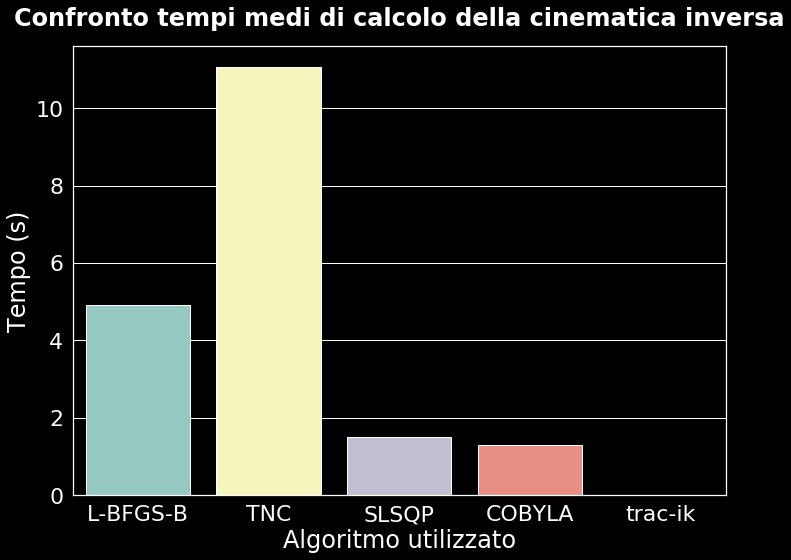
\includegraphics[width=\textwidth]{slide/img_cinematica_inversa/risultati_tempi.png}
\end{column}
\end{columns}

\note{
I tempi medi migliori si hanno sugli algoritmi SLSQP e COBYLA. Gli altri scartati. 

TRAC-IK ha timeout.
}
\end{frame}

\begin{frame}{Valutazione degli algoritmi: errore sulla posizione}
\begin{columns}
\begin{column}{0.3\textwidth}
Errore percentuale sulle soluzioni del \emph{Problema 1} su un campione di 200 punti uniformemente distribuiti nello spazio raggiungibile.
\end{column}
\begin{column}{0.7\textwidth}
\hspace*{-2em}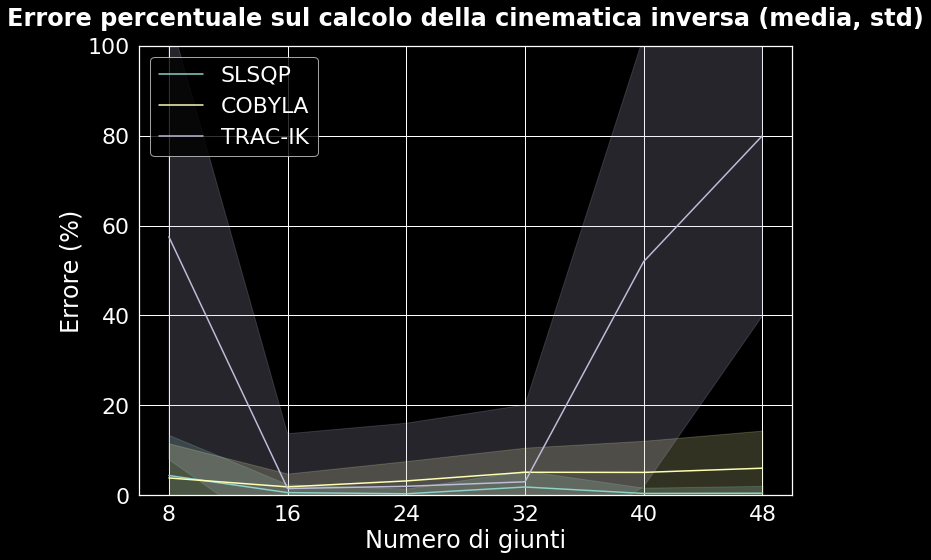
\includegraphics[width=1.15\textwidth]{slide/img_cinematica_inversa/risultati_errore.png}
\end{column}
\end{columns}

\note{
Errore SCIPY costante con i due algoritmi considerati. Errore maggiore con 8GDL.

TRAC-IK molto bene con >16, <32 e molto male altrove. 
}

\end{frame}

\begin{frame}{Valutazione degli algoritmi: accuratezza punti}
\begin{columns}
\begin{column}{0.35\textwidth}
\end{column}
\begin{column}{0.7\textwidth}
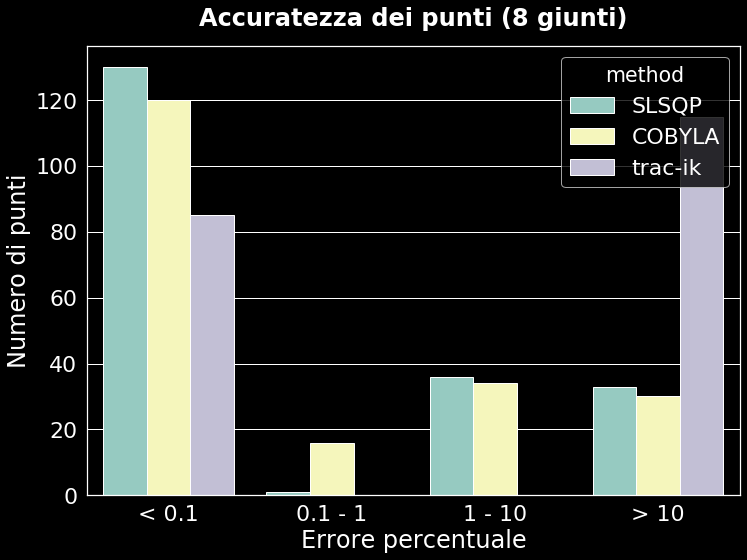
\includegraphics[width=\textwidth]{slide/img_cinematica_inversa/accuratezza_8.png}
\end{column}
\end{columns}

\note{
Accuratezza: 8gdl così così SCIPY (1\%-10\%), male TRAC-IK. 
}
\end{frame}

\begin{frame}{Valutazione degli algoritmi: accuratezza punti}
\begin{columns}
\begin{column}{0.35\textwidth}
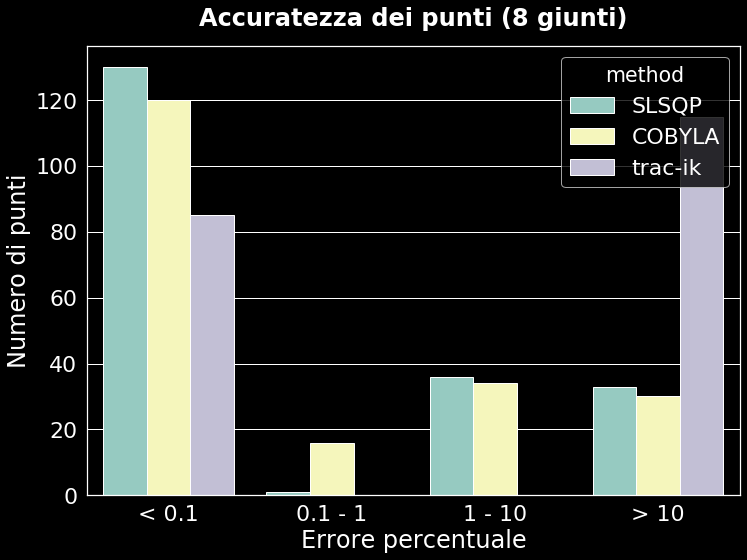
\includegraphics[width=\textwidth]{slide/img_cinematica_inversa/accuratezza_8.png}

\hfill

\end{column}
\begin{column}{0.7\textwidth}
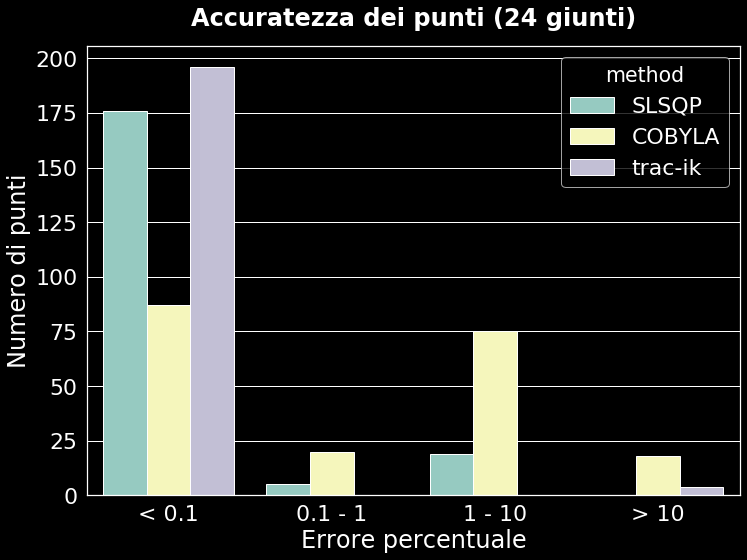
\includegraphics[width=\textwidth]{slide/img_cinematica_inversa/accuratezza_24.png}
\end{column}
\end{columns}

\note{
24 gdl TRAC-IK benissimo. 
}
\end{frame}

\begin{frame}{Valutazione degli algoritmi: accuratezza punti}
\begin{columns}
\begin{column}{0.35\textwidth}
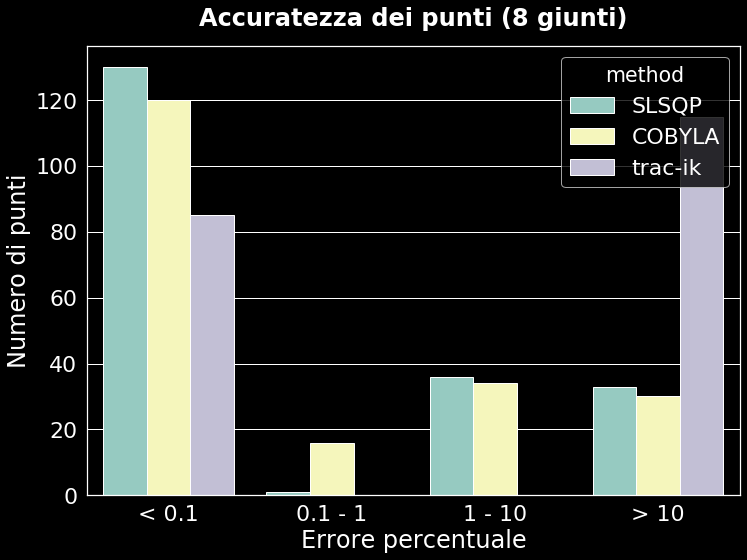
\includegraphics[width=\textwidth]{slide/img_cinematica_inversa/accuratezza_8.png} 

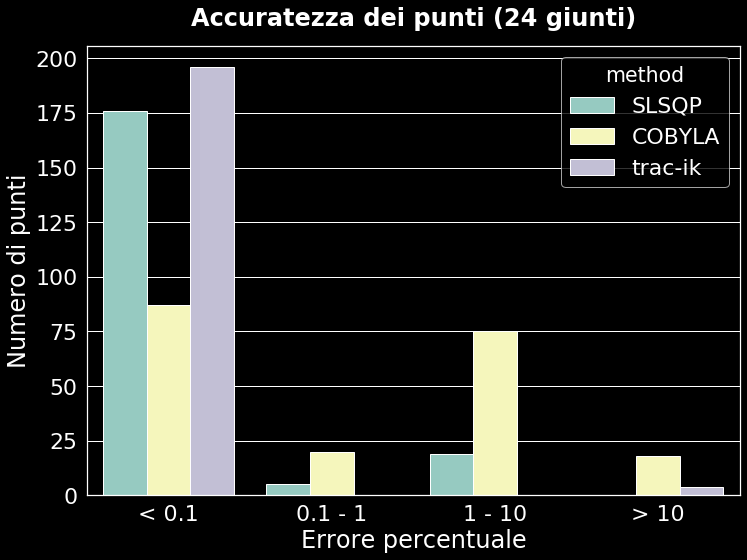
\includegraphics[width=\textwidth]{slide/img_cinematica_inversa/accuratezza_24.png}

\hfill
\end{column}
\begin{column}{0.7\textwidth}
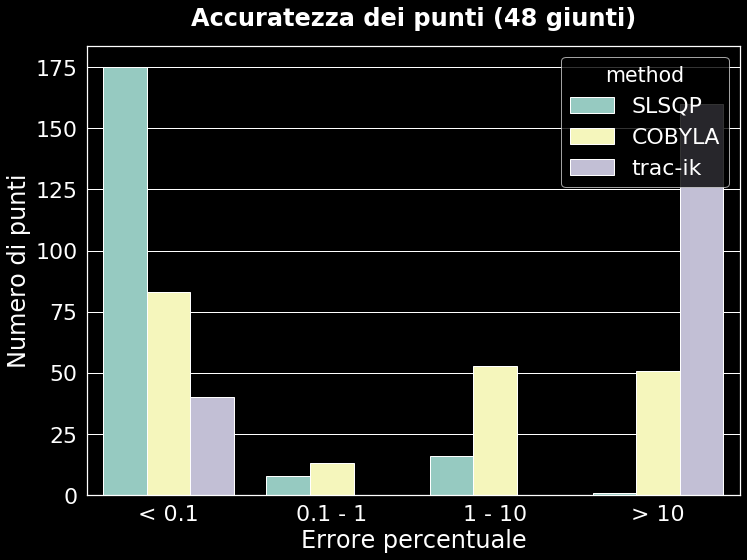
\includegraphics[width=\textwidth]{slide/img_cinematica_inversa/accuratezza_48.png}
\end{column}
\end{columns}
\note{
48 gdl TRAC-IK malissimo. 
}
\end{frame}

\begin{frame}{Valutazione degli algoritmi: \emph{Problema 2}}
\begin{columns}
\begin{column}{0.55\textwidth}
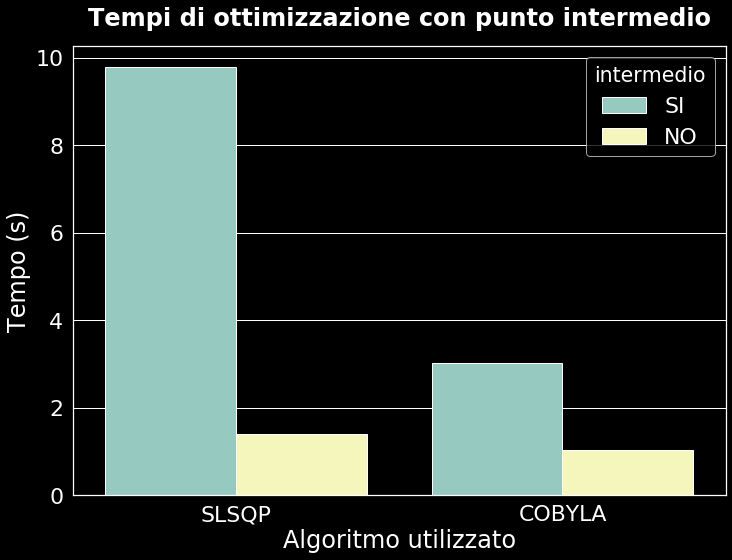
\includegraphics[width=\textwidth]{slide/img_cinematica_inversa/intermedio_tempi.png} 
\end{column}
\begin{column}{0.55\textwidth}
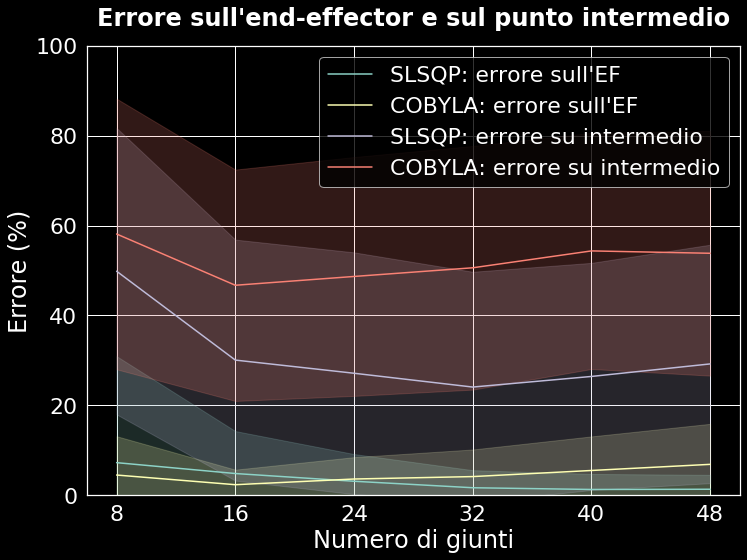
\includegraphics[width=\textwidth]{slide/img_cinematica_inversa/intermedio_errore.png}
\end{column}
\end{columns}
\note{
Non posso confrontare con TRAC-IK poichè non considera punti intermedi. 

Performance temporali SLSQP x5, COBYLA x2. Errore end effector aumenta. Errore punto intermedio alta: posso davvero raggiungere tale il punto principale passando da quello intermedio? Sono generati a caso...
}
\end{frame}

\begin{frame}{Risultati}
\begin{itemize}
\item<1-> TRAC-IK: ottimo con manipolatori di 16-32 giunti 
\includegraphics[width=10px]{slide/img_cinematica_inversa/hundred_point_emoji.png}
\item<2-> SCIPY + SLSQP valida alternativa a TRAC-IK con più di 32 giunti
\begin{itemize}
    \item[\leftthumbsup] posso dare forma al manipolatore
    \item[\leftthumbsdown]<3-> tempi piuttosto lunghi
\end{itemize}
\end{itemize}

\note{
L'approccio proposto da TRAC-IK è ottimo per un numero di giunti compreso tra 16 e 32, sia per i tempi che per l'errore.

Con più di 32 giunti l'approccio migliore è l'algoritmo SLSQP di SCIPY che permette anche di dare forma al manipolatore.

I tempi sono piuttosto lunghi, introdurre un timeout.
}
\end{frame}
\TransitionFrame{fine}

\end{document}
